\labelsubsection{Results and Observations}{subsec:results_and_observations}
In the next paragraphs we will investigate the questions we posed in the previous chapter.
After that, we will gather the findings to these questions to form an answer to our main hypothesis.

\todo[inline]{Observations + possible explanations}
\todo[inline]{How do the results relate to hypothesis?}
\todo[inline]{Error analysis}
\todo[inline]{Comparison between text n-grams and concept maps/co-occurrence graphs}
\todo[inline]{Look at concepts used in concept maps: frequency in whole corpus, ...}

\subquestionref{question:structure_diversity}
To investigate whether concept maps are useful for text classification, we first look at the structure of concept maps.
The structure of concept maps is the main difference to most plain text representations.
Finding out whether the structures of concept maps are heterogeneous is therefor a first crucial step in understanding the usefulness of concept maps.

In Figure \ref{fig:graph_statistics}, we gathered metrics about the connectedness of concept maps and co-occurrence graphs with window size 1 for comparison.
One thing that immediately becomes apparent is the compression factor of the concept maps: on average, only approximately 8\% of the original text-content is retained in the concept maps.
This compression is useful for tasks like text summarization where only important concepts should be kept from the underlying text.

One consequence of this compression can be seen when looking at the connectedness of the concept maps.
On average, concept maps have only 1.36 edges per node. The minimum number of edges per node is 1 since we removed all unconnected nodes.
So, concept maps do not only have few nodes but also a relatively low number of edges between them.
This is most likely due to the small length of the underlying texts.
The shortness of the text results in a lower number of occurrences of some concept in the text, ie. most of the concepts occur only once in a text.

Another hint for the un-connectedness of concept maps is the number of connected components.
In Figure \ref{fig:percentage_more_than_one_connected_component} we can see that most of the graphs have more than one connected component. Together with the observation of the low number of nodes per graph, this also implies the low connectedness of concept maps.
In Figure \ref{fig:histogram_connected_components} we also plotted the histogram of the number of connected components per graph which also confirms the hypothesis that concept maps are fairly un-connected.

In Figure \ref{fig:graph_examples} shows examples of concept maps and co-occurrence graphs with different window sizes.

\begin{figure}[ht]
\centering
\begin{tabular}{lcccccc}
{} &  \multicolumn{2}{c}{\#nodes/\#words} &  \multicolumn{2}{c}{\#edges/\#nodes} & \multicolumn{2}{c}{\#nodes/graph} \\
{} & concept map &  co-occurrence & concept map & co-occurrence & concept map & co-occurrence\\
\midrule
ling-spam       & 0.05 & 0.23 & 1.32 & 2.86 & 45.95 & 4.11 \\
ng20            & 0.05 & 0.18 & 1.38 & 2.71 & 584.63 & 87.52 \\
reuters-21578   & 0.09 & 0.21 & 1.46 & 2.86 & 63.07 & 13.20 \\
review\_polarity & 0.08 & 0.20 & 1.42 & 2.67 & 50.36 & 10.55 \\
rotten\_imdb     & 0.09 & 0.30 & 1.22 & 1.70 & 52.09 & 11.23 \\
tagmynews       & 0.13 & 0.37 & 1.30 & 1.81 & 52.74 & 13.25 \\
webkb           & 0.05 & 0.22 & 1.39 & 3.01 & 55.69 & 5.36 \\
\midrule
\O{}            & 0.08 & 0.24 & 1.36 & 2.52 & 129.22 & 20.75 \\
\bottomrule
\end{tabular}
\caption{Graph statistics. \textit{\#words} is the number of words in the whole text dataset. The \textit{\#edges/\#nodes} metric is for the co-occurrence graphs with a window size of 1. The \textit{\#nodes/\#words} metric is a compression factor. Note that, on average, the concept maps have a compression factor of 8\% compared to the 24\% of the co-occurrence graph. This means that co-occurrence graphs have approximately three times more content than concept maps. The \textit{\#edges/\#nodes} metric is an indicator for the connectedness of the graphs. Because we remove nodes which have no edge to other nodes, the \textit{\#edges/\#nodes} metric captures the average degree of the nodes. Looking at that metric we also see that, on average, the co-occurrence graphs with window size 1 have roughly twice as much edges per node as concept maps.}\label{fig:graph_statistics}
\end{figure}

\begin{figure}[ht]
\centering
\centering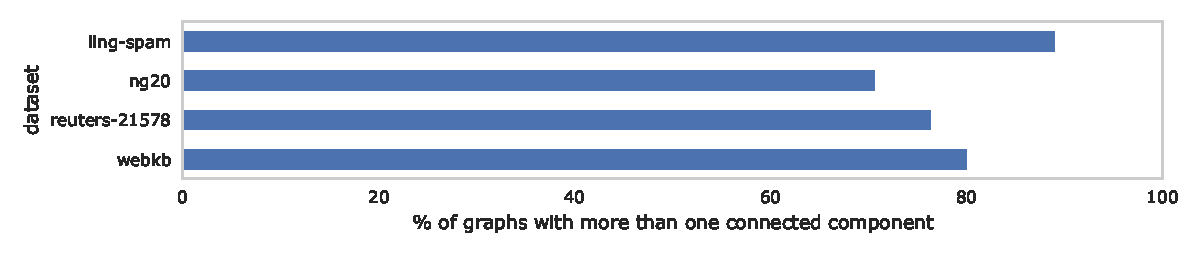
\includegraphics[width=1\linewidth]{assets/figures/percentage_more_than_one_connected_component.pdf}
\caption{Percentage of graphs with more than one connected component. TODO: This can also be put into a table!}\label{fig:percentage_more_than_one_connected_component}
\end{figure}

\begin{figure}[ht]
\centering
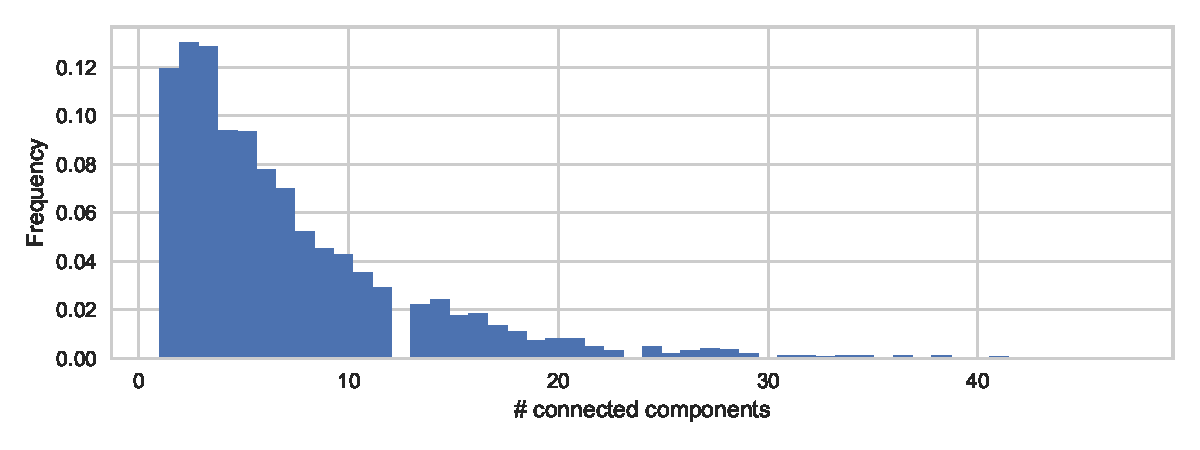
\includegraphics[width=0.8\linewidth]{assets/figures/hist-connected-components-ling-spam-CMap.pdf}
\caption{Histogram of connected components per concept map. Dataset: ling-spam.}\label{fig:histogram_connected_components}
\end{figure}

\begin{figure}[ht]
\centering
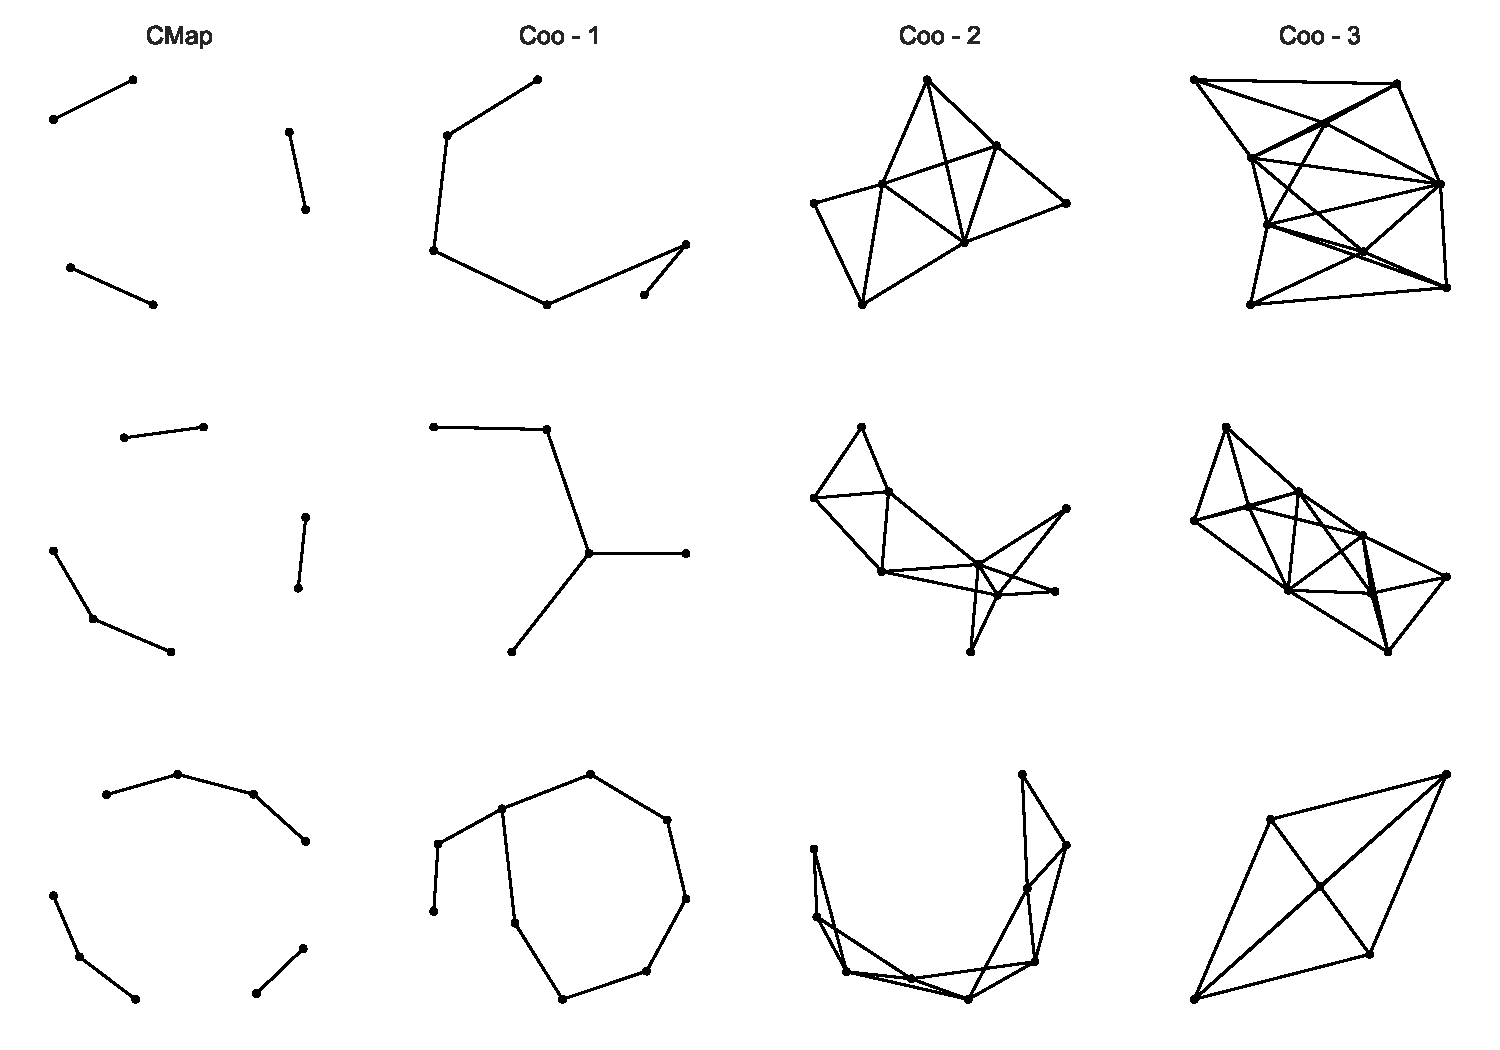
\includegraphics[width=0.6\linewidth]{assets/figures/graph-examples.pdf}
\caption{Graph examples per type. Three examples are shown per type. The number after the co-occurrence graph label signify the window size. The concept map examples all have more than one connected component, while the co-occurrence graphs all have only one. Taken from the \textit{ling-spam} dataset.}\label{fig:graph_examples}
\end{figure}

\begin{figure}[ht]
\centering
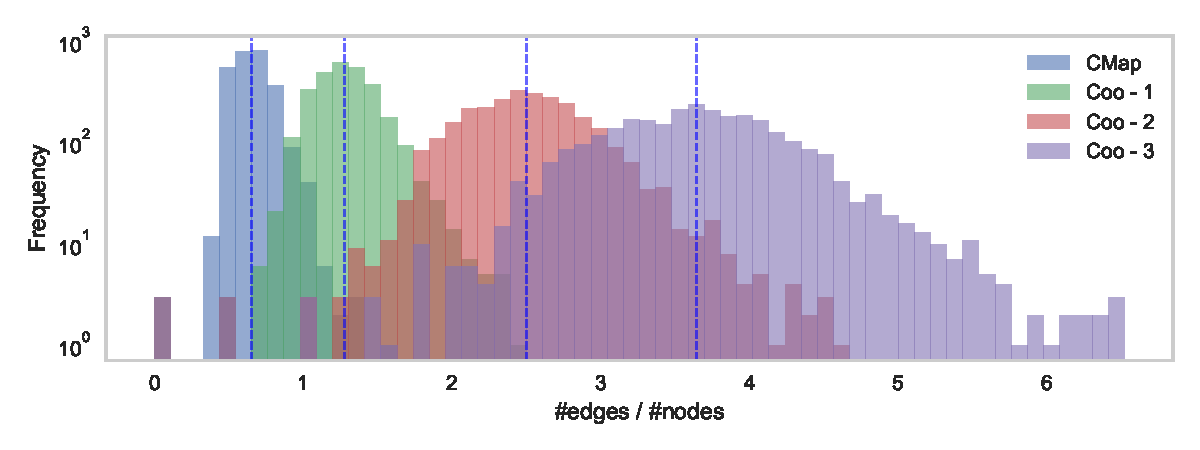
\includegraphics[width=0.7\linewidth]{assets/figures/hist-edgesnodes.pdf}
\caption{Histogram of the number of edges divided by the number of nodes. Per graph type. The lines correspond to the median value.}
\label{fig:histogram-edges-div-nodes-per-type}
\end{figure}

The co-occurrence graphs have a relatively simple structure.
Co-occurrence graphs are always connected, ie. the number of connected components is 1, or 0 in the case of an empty graph.
When the window size is 1, the graph is similar to a path, meaning that most of the nodes have a degree $< 2$. With increasing window size, the graph gets more connected.


\subquestionref{question:importance_structure}
\begin{figure}[ht]
\centering
\missingfigure[figcolor=white]{}
\caption{Comparison of linearized graph with CountVectorizer and results of WL}
\end{figure}

\begin{figure}[ht]
\centering
\missingfigure[figcolor=white]{}
\caption{Comparison of WL with and without labels}
\end{figure}

\subquestionref{question:comparison_coo}
\begin{figure}[ht]
\centering
\missingfigure[figcolor=white]{}
\caption{Comparison of co-occurrence results with concept maps}
\end{figure}

\subquestionref{question:comparison_text}
\begin{figure}[ht]
\centering
\missingfigure[figcolor=white]{}
\caption{Comparison of concept maps with text}
\end{figure}

\subquestionref{question:comparison_combined}
\begin{figure}[ht]
\centering
\missingfigure[figcolor=white]{}
\caption{Comparison of classification using both concept maps and text}
\end{figure}



\labelsubsection{Related And Intermediate Observations}{subsec:related_and_intermediate_observation}
\todo[inline]{Sparsity of feature vectors}
\todo[inline]{Complexity of approach}